\documentclass[a4paper]{article}

%% Language and font encodings
\usepackage[english]{babel}
\usepackage[utf8x]{inputenc}
\usepackage[T1]{fontenc}
\usepackage{graphicx}
\usepackage{float}
\usepackage{amsmath}

%% Sets page size and margins
%\usepackage[letter,top=3cm,bottom=2cm,left=3cm,right=3cm,marginparwidth=1.75cm]{geometry}

%% Useful packages
\usepackage{amsmath}
\usepackage{graphicx}
\usepackage[colorinlistoftodos]{todonotes}
\usepackage[colorlinks=true, allcolors=blue]{hyperref}

\title{CS534 - Implementation Assignment 3}
\date{\today}
\author{Peter Rindal, Hung Viet Le, and Trung Viet Vu}

\begin{document}
\maketitle

%\section{Group Information}
\begin{center}
  \begin{tabular}{ | c | c | c | }
    \hline
    Member Name & OSU ID & Contribution \\ \hline
    Peter Rindal & 931731553 & 33.33\% \\ \hline
    Hung Viet Le & 932259606 & 33.33\% \\ \hline
    Trung Viet Vu & 932986775 & 33.33\% \\
    \hline
  \end{tabular}
\end{center}

\section{Decision trees and Random forest}


\subsection{Implement a decision tree algorithm}
\begin{enumerate}
\item[(a)] For calculating threshold of each feature in this implementation, we divide each feature's range into equal parts and compute the information gain (IG) for each milestone. %Note that we do not use the method mentioned in the class: only choose thresholds on feature values that class label changes.
\item[(b)] Below is the figures for each threshold and each feature at the root node with k=8. Only thresholds with unique IG are reported.

\begin{figure}[H]
\begin{center}
\includegraphics[width=5in]{thresholds.png}
\caption{Information Gain of each threshold and each feature for the root node}
\end{center}
\end{figure}


\item[(c)]


\begin{figure}[H]
	\begin{center}
		\includegraphics[width=5in]{minSPlitVsK.pdf}
		\caption{Accuracy on test data for different values of $k$.}
	\end{center}
\end{figure}



\item[(d)] When $k$ is too small, the tree model will over fit the training data. When $k$ is too large, it will under learn and prevent the model from taking advantage of differences that effect only a small set of nodes in the training set.


\end{enumerate}



\subsection{Random Forest}
\begin{enumerate}
	\item[(d)] $ $
	
	\begin{figure}[H]
		\begin{center}
			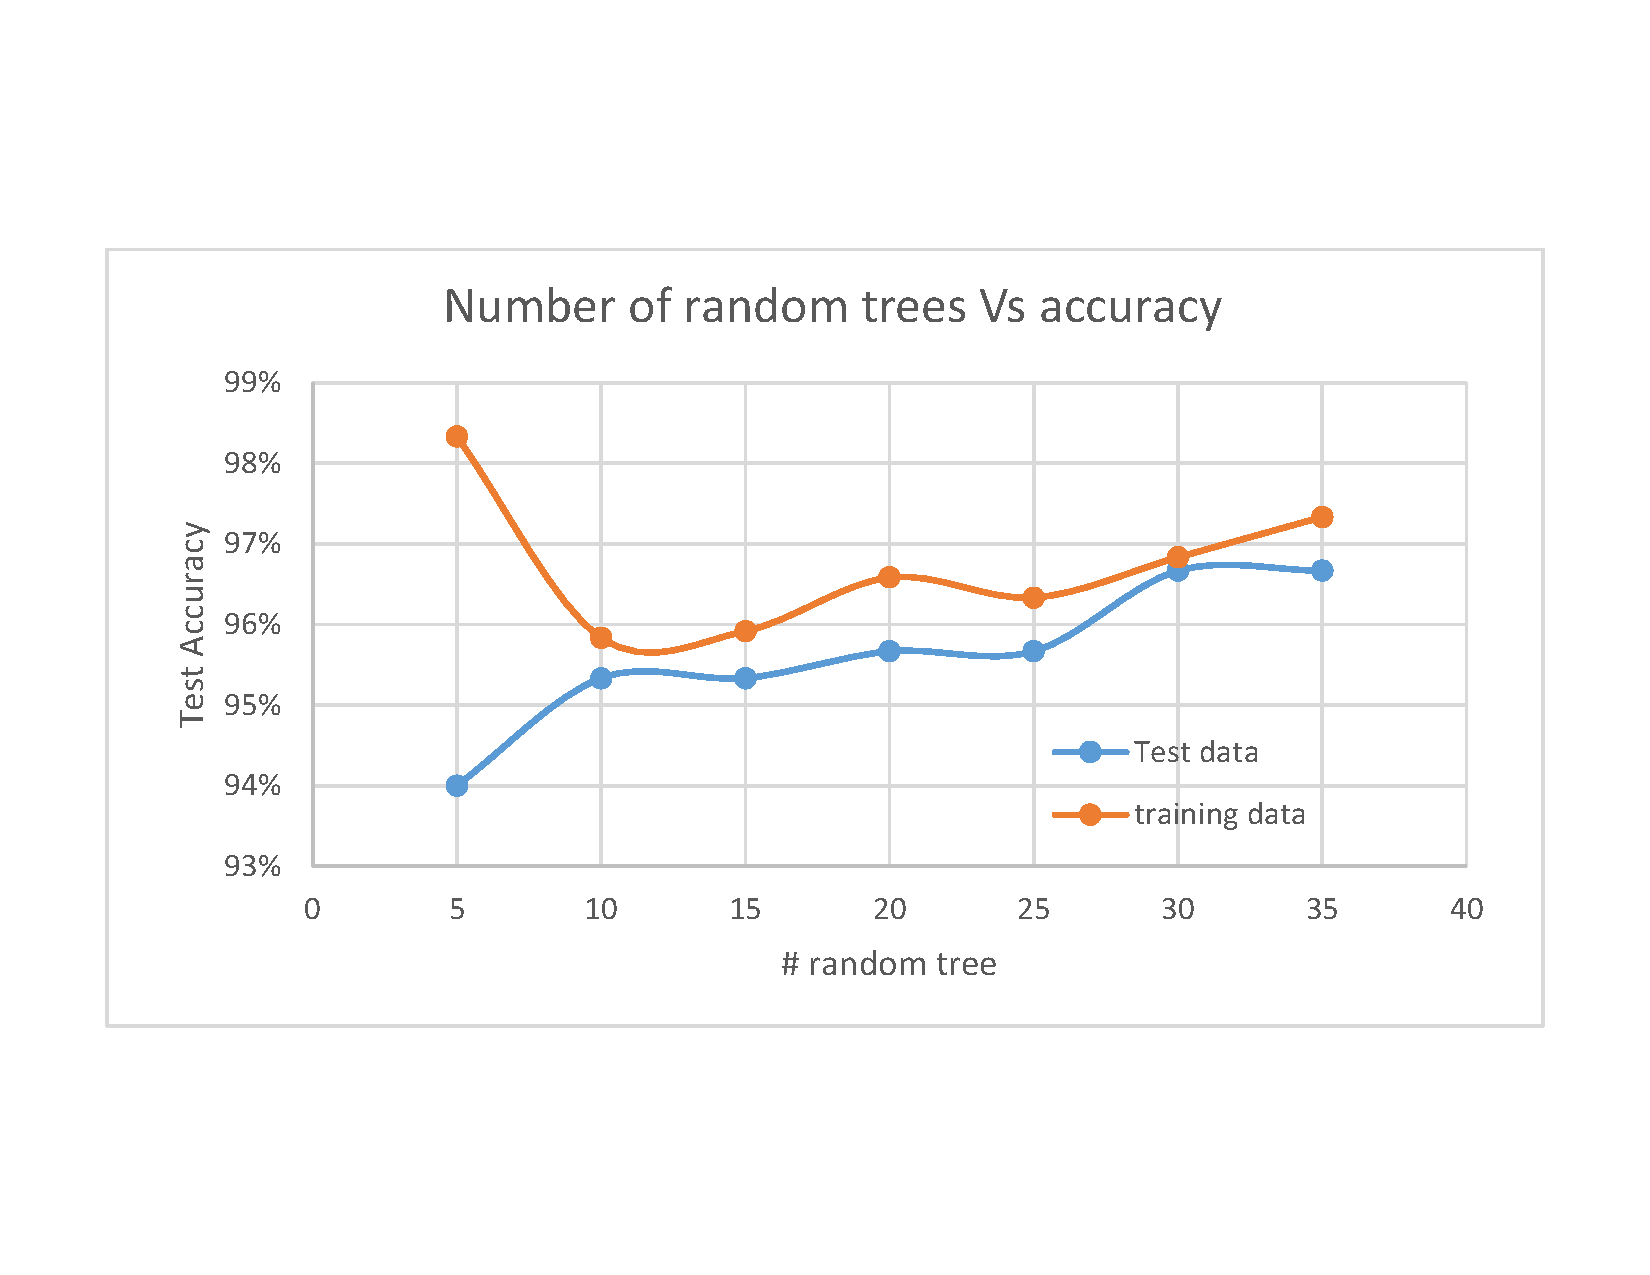
\includegraphics[width=5in]{random.pdf}
			\caption{Accuracy on test data for number of random trees.}
		\end{center}
	\end{figure}
	
\item[(e)] We observed that the training data was much more accurate in general (over fitting). This was especially true when the min node size was small. In this case the model would almost always predict everything in the training set with high accuracy. In the case that we added more random tree, with all of their randomizations, we observed that this over fitting decreased. This was especially true when $k$ was large. However, it was somewhat hard to detect because our models were already highly accurate, roughly 90+ percent for a large portion on the parameters.

In addition to reducing the over fitting of the training set, adding more trees increased the accuracy of the test dataset. However, when using reasonable parameters, we saw minimal impact of random feature selection. While it did help some when we ran many trials or had many trees, overall its impact was minimal. 

When using many trees, found that we got the best result when $k$ was around 5. We believe this is 5 allows the algorithm to tune into the data enough while still preventing too much overfitting. We also found that when using enough trees and the random feature selection, a larger $k$ value also obtains good results.

	
\end{enumerate}
\end{document}
















